
At the core of many numerical PDE solution methods is the solution of a finite-dimensional linear system.  Because such linear systems become more-accurate representations of the PDE as their size goes to infinity, one tends to solve the largest linear systems which the available computing technology can handle.  Solving such linear systems, using algorithms that have the potential to scale to very large sizes---so large, for instance, that the vector solution of the system must be distributed across many processors to even fit in memory---represents the core technology in \PETSc.

This Chapter starts by reviewing the basic ideas of numerical linear algebra, but we move relatively fast; the review is finished by page \pageref{subsec:ls:vecmatintro}.\sidenote{\citet{TrefethenBau1997} is thus recommended as a textbook-length treatment.}  Our goal, besides stating elementary definitions, is to identify the fundamental constraints which makes solving large systems challenging.  Thus we assert several ``facts of life'' about the process.  Then the central threads of iterative linear algebra are laid out, namely iteration to reduce the residual, preconditioning to improve the convergence of the iteration, and the ``Krylov space'' idea, and its connection to polynomial approximation, to unify iterative schemes under one (generous) umbrella.

We then introduce the \PETSc types for storing vectors and matrices.  We apply \PETSc to solve a small linear system.  This is followed by a somewhat more-representative example of a sparse, arbitrary-size, tridiagonal system.  The latter example is exploited for a first look at the comparative effectiveness of the run-time options which choose Krylov-space and preconditioner methods.


\section{Vector spaces, matrices, and norms}

Vector spaces, matrices, and norms are assumed to be familiar to the reader, but we can set some notation by recalling the basics.

A \emph{real vector space} is a set that is closed under addition and multiplication by \emph{scalars} (elements of $\RR$)\sidenote{\PETSc can be configured to handle complex scalars, vectors, and matrices.  However, in this book we use only real numbers.} and to which certain algebraic axioms apply.\sidenote{Namely, the existence of a zero vector plus the appropriate associative, distributive, and commutative axioms \citep{Strang2009}.}  The elements of the set are \emph{vectors}.

The unqualified word ``vector'' will be understood in this book to refer to a column vector of finite length.  The space of such vectors of length $N$ is written $\RR^N$.  On the other hand we will also regard functions defined on domains in $\RR^d$, where $d=1,2,3$, as vectors in infinite-dimensional vector space.  The solutions to PDEs live in such spaces.

We will use bold for vectors, but not for entries, thus for example $\bv\in\RR^N$ has entries $v_0,\dots,v_{N-1}\in \RR$; we break tradition by numbering vector entries starting from zero.  The \emph{standard basis} for $\RR^N$ is the set of vectors $\{\be_i\}_{i=0}^{N-1}$ which are zero except for a one in the $i$th entry: $(\be_i)_j = \delta_{ij}$ (the Kronecker delta).

A \emph{matrix} is a linear map between vector spaces.\sidenote{In polite company one says instead that a matrix is the \emph{representation} of a linear map from one finite-dimensional vector space to another, with some choice of basis in each space.}  We write $A\in \RR^{M\times N}$ for a matrix that maps from $\RR^N$ to $\RR^M$.  There are two related matrices which map in the other direction.  If the matrix is square and invertible then the \emph{inverse} $A^{-1}\in \RR^{N\times M}$ is the unique matrix satisfying $A^{-1} A = A A^{-1}=I$.  Even if $A$ is non-square one can construct $A^\top\in \RR^{N\times M}$, namely the \emph{transpose} with entries $(A^\top)_{ij}=a_{ji}$.

A \emph{vector norm} is a function $\|\cdot\|:\RR^N \to [0,\infty)$ which assigns a well-defined length to a vector.\footnote{Several axioms, including the triangle inequality, must be satisfied \citep{TrefethenBau1997}.}  For $1 \le p < \infty$ this formula defines a norm,
\begin{equation}
\|\bv\|_p = \left(\sum_{i=0}^{N-1} |v_i|^p\right)^{1/p}.  \label{eq:ls:vectorpnorm}
\end{equation}
The $p=1,2$ cases are especially common in practical use, but all vector $p$-norms can be computed with $O(N)$ work.  The maximum norm, which is also the $p\to\infty$ limit of \eqref{eq:ls:vectorpnorm}, is equally wide-spread:
\begin{equation}
\|\bv\|_\infty = \max_{i=0,\dots,N-1} |v_i|.  \label{eq:ls:vectorinfnorm}
\end{equation}
Note that \PETSc computes the $p=1,2,\infty$ vector norms by a call to \texttt{VecNorm()} on a \PETSc \pVec object; these are introduced below.

Choosing vector norms on the input and output vector spaces of a matrix \emph{induces} a \emph{matrix norm} \citep{TrefethenBau1997}, as follows:
\begin{equation}
\|A\| = \sup_{\bv \ne 0} \frac{\|A\bv\|}{\|\bv\|} = \sup_{\|\bv\| = 1} \|A\bv\|.  \label{eq:ls:matnorm}
\end{equation}
It follows from \eqref{eq:ls:matnorm} that
    $$\|A \bv\| \le \|A\| \|\bv\|.$$

Generally, induced matrix norms are expensive to compute.  In most of the cases, they are optimization problems which take more work than the $O(MN)$ operations needed to examine all the entries of a (generic, dense) matrix $A\in \RR^{M\times N}$.  However, the matrix norms induced by the $p=1$ and $p=\infty$ vector norms are easy to compute by $O(MN)$ formulas \citep{TrefethenBau1997}.  The \emph{Frobenius} matrix norm can also be computed by a $O(MN)$ formula, though this norm is not induced from a vector norm \citep{TrefethenBau1997}.  Thus it is that \PETSc can compute $p=1,\infty$ and Frobenius matrix norms by a call to \texttt{MatNorm()} on a \PETSc \pMat object (see below), but not other induced norms.

We will use vector norms routinely in practice, both inside key algorithms for linear and nonlinear analysis (Chapters \ref{chap:ls}, \ref{chap:st}, \ref{chap:nl}), and in measuring numerical errors in solving PDEs, for example.   But what good are matrix norms?  In this book we will use them only through the desire to measure the \emph{conditioning} of linear systems \citep{TrefethenBau1997}.  By definition, if $\|\cdot\|$ denotes a matrix norm and $A \in \RR^{N\times N}$ is a square matrix then
\begin{equation}
    \kappa(A) = \|A\| \|A^{-1}\|  \label{eq:ls:conddefn}
\end{equation}
is the \emph{condition number} of $A$.  (By definition $\kappa(A)=+\infty$ if $A$ is not invertible.)  This quantity measures how sensitive the (exact) solution of a linear system $A \bv = \bb$ is to perturbations of either the matrix $A$ or the right-hand-side $\bb$ \citep{TrefethenBau1997}.


\section{Linear systems, and some facts of (numerical) life}

Suppose $\bb\in \RR^{N}$ is a column vector and $A\in\RR^{N\times N}$ is a square matrix.  The linear system
\begin{equation}
A \bu = \bb \label{introsystem}
\end{equation}
has a unique solution $\bu\in \RR^{N}$ if $A$ is invertible, namely
\begin{equation}
\bu = A^{-1} \bb. \label{introsolution}
\end{equation}
This is simple in theory.

It is not so simple in practice, however, to solve linear systems on a computer.  Here are three facts to keep in mind while working numerically with linear systems \citep{TrefethenBau1997}:
\renewcommand{\labelenumi}{Fact \Roman{enumi}.}
\begin{enumerate}
\item \label{page:ls:limittoaccuracy} \emph{There is an unavoidable limit to numerical accuracy.}  If real numbers are represented with machine precision $\eps$ then the solution of \eqref{introsystem} can only be computed within an error $\kappa(A) \eps$, where $\kappa(A)$ is the \emph{condition number} of $A$.
\item \emph{Direct solutions may have a high cost.}  For a generic, dense $N\times N$ matrix $A$, computation of the solution to \eqref{introsystem}, by a direct method such as Gauss elimination \citep{TrefethenBau1997}, whether actually forming $A^{-1}$ or not, is an $O(N^3)$ operation.\sidenote{See Lecture 32 in \citet{TrefethenBau1997} for caveats with respect to ``$O(N^3)$.''  Nonetheless it is the right power to state when making this point.}
\item \emph{Generally you should not form the inverse.}  The matrices $A$ arising from discretized PDEs are usually sparse, but their inverses $A^{-1}$ are usually dense and may not even fit in memory.
\end{enumerate}

Fact I is about conditioning not methods.  Informally speaking, there are matrices $A$ and $\tilde A$ that are the same to within machine precision $\eps$ but for which the exact solutions to \eqref{introsystem} using $A$ and $\tilde A$ differ by an amount $\kappa(A) \eps$.  Rounding errors, which act somewhat like random noise added to every arithmetic operation on the computer, effectively perturb $A$ by $\eps$ during each computation, and thus $O(\kappa(A) \eps)$ size errors appear in the solution of the linear system.  \emph{Backward stable} methods, specifically the QR direct method, can be shown to essentially achieve this minimal level of inaccuracy \citep{TrefethenBau1997}.

The precision for the C \texttt{double} type, the default 64-bit representation of real numbers,\sidenote{This type is aliased to \texttt{PetscReal} and \texttt{PetscScalar} in most \PETSc configurations.} is $\eps = 2.2 \times 10^{-16}$.  Thus by i), a linear system having $\kappa(A) \approx 10^{10}$, for example, can only be solved to five or six decimal digits of precision.  Indeed it is possible to see $\kappa(A)\approx 10^{10}$ for $A$ which come from discretizing a PDE, but such a matrix is regarded as ``poorly-conditioned.''  We would normally inquire whether different discretization choices might generate a new matrix with a smaller condition number.  In any case, expectations about solution accuracy should be informed by estimates of matrix condition numbers.

By Fact II, a generic linear system with $N=10^6$ equations requires $10^{18}$ or so operations to solve by Gauss elimination, and even modern supercomputers take a while to do a quintillion operations.  However, though general-purpose direct methods are impractical for most $N=10^6$ systems, we will successfully solve PDE-generated linear systems of this size on a single processor in a few seconds, and in $O(N)$ operations, using (non-direct) iterative methods (Chapters \ref{chap:st}, \ref{chap:pr}).

A key idea is that discretized PDEs generate linear systems with exploitable structure, especially \emph{sparsity}, which means that there are few nonzero entries per matrix row.  For the methods to converge there also needs to be other structure in the linear system such as regularity of the matrix entries arising from the smoothness of the coefficients in the PDE.  This structure will be exploited, and exposed to one degree or another, in serious numerical PDE solutions.  Naive application of direct methods---treating solvers for \eqref{introsystem} as unadjusted black boxes---is too slow.

For simple example illustrating Fact III, the $N$-dimensional tridiagonal matrix $A$ assembled later in this section occupies $24 N$ bytes, because each allocated real entry occupies 8 bytes using double precision.  The inverse $A^{-1}$, however, is dense and uses $8 N^2$ bytes.  Though we can easily solve $A\bu=\bb$ for this matrix in dimension $N=10^7$, using less than a gigabyte of memory in the solution process,\sidenote{See \texttt{tri.c}.  Do ``\texttt{./tri -tri\_m 10000000 -ksp\_type cg -pc\_type none}.''} simply storing $A^{-1}$ would occupy $800$ terabytes of memory or disk.


\section{Iterative linear algebra 1: residual and iterations}

Direct methods like Gauss elimination \citep{TrefethenBau1997} are one way to solve a linear system.  The most powerful methods for solving PDEs, however, are iterative.

By definition, the \emph{residual} of $\bu_0$ in linear system \eqref{introsystem} is the vector
\begin{equation}
\br_0 = \bb - A \bu_0. \label{residualdefn}
\end{equation}
Evaluating the residual for a known vector $\bu_0$ requires only applying $A$ to it, an $O(N^2)$ operation at worst.  Because most discretization schemes for PDEs generate matrices $A$ that are \emph{sparse}, with many more zero entries than nonzeros, and because often the number of nonzeros per row is typically small and independent of $N$, the product $A\bu_0$ can often be computed in $O(N)$ operations.

The \emph{Richardson iteration},\sidenote{Also called \emph{simple iteration} \citep{Greenbaum1997}.} simply adds a multiple $\omega$ of the last residual at each step,
\begin{equation}
\bu_{k+1} = \bu_k + \omega (\bb - A \bu_k).  \label{introrichardson}
\end{equation}
If significantly fewer than $O(N^2)$ steps were needed to make $\bu_k$ an adequate approximation of the exact solution $\bu$, then the Richardson iteration could improve on Gauss elimination.  In many cases the Richardson iteration may not converge, as in the next Example.

\medskip\noindent\hrulefill
\begin{example} Consider the linear system
\begin{equation}
A \bu
= \begin{bmatrix}
10 & -1 \\ -1 & 1
\end{bmatrix}
\begin{bmatrix} u_1 \\ u_2 \end{bmatrix}
= \begin{bmatrix} 8 \\ 1 \end{bmatrix}
= \bb
 \label{introexample}
\end{equation}
which has solution $\bu = [1\,\, 2]^\top$.  If we start with estimate $\bu_0 = [0\,\, 0]^\top$ then the $\omega=1$ Richardson iteration \eqref{introrichardson} gives a sequence of vectors % see ../matlab/richardsonex.m
\begin{equation}
\rvect{0}{0}{0}, \rvect{1}{8}{1}, \rvect{2}{-63}{9}, \rvect{3}{584}{-62}, \dots
\end{equation}
This sequence is not heading toward the solution.
\end{example}
\noindent\hrulefill

\medskip
If we rewrite \eqref{introrichardson} as
\begin{equation}
\bu_{k+1} = (I - \omega A) \bu_k + \omega \bb  \label{introrewriterichardson}
\end{equation}
then it is easy to believe that the ``size'' of the matrix $I-\omega A$ will determine whether $\lim_{k\to\infty} \bu_k$ exists.  To give a precise meaning to this statement we recall important definitions.

A complex number\sidenote{Though $B$ is real, $\lambda$ may be complex.} $\lambda \in \CC$ is an \emph{eigenvalue} of a square matrix $B\in\RR^{N\times N}$ if there is a nonzero vector $\bv\in\CC^N$ so that $B \bv = \lambda \bv$.  The set of all eigenvalues of $B$ is the \emph{spectrum} $\sigma(B)$ of $B$.  The \emph{spectral radius} $\rho(B)$ is the maximum magnitude of the eigenvalues of $B$.  The \emph{singular values} are the square roots of the eigenvalues of the matrix\sidenote{This matrix is always symmetric and it is either positive-definite or positive semi-definite.  Thus it has nonnegative eigenvalues.} $B^\top B$.  Singular values are geometrically-defined as the lengths of semi-axes of the (hyper-)ellipsoid in $\RR^N$ that results from applying $B$ to all vectors in the unit (hyper-)sphere of $\RR^N$ \citep{TrefethenBau1997}.

Properties of a matrix described in terms of its eigenvalues or singular values are generically called ``spectral properties.''  For example, $\|B\|_2$ is the largest singular value of $B$ and $\|B^{-1}\|_2$ is the inverse of the smallest singular value of $B$, so these are spectral properties.  The 2-norm condition number $\kappa(B)=\|B\|_2/\|B^{-1}\|_2$ is thus also a spectral property; it is visualized as the eccentricity of the ellipsoid above.

Exercise \ref{chap:ls}.\ref{exer:ls:showconvergethm} asks you to show that the Richardson iteration \eqref{introrichardson} or \eqref{introrewriterichardson} will converge if and only if all the eigenvalues of $B=I-\omega A$ are inside the unit circle:
\begin{equation}
\text{\eqref{introrichardson} converges if and only if } \rho(I-\omega A) < 1. \label{introconvergethm}
\end{equation}
One can also show that $\rho(B) \le \|B\|$ in any induced matrix norm, so that \eqref{introrichardson} converges if $\|I-\omega A\| < 1$.


\section{Iterative linear algebra 2: preconditioning}

Considering spectral properties brings us to an important general observation about linear systems.  Namely, that there are many systems which are equivalent to \eqref{introsystem}.  In fact, if $M\in\RR^{N\times N}$ is an invertible matrix then the systems
\begin{equation}
(M^{-1} A) \bu = M^{-1} \bb \label{introleftpre}
\end{equation}
and
\begin{equation}
(A M^{-1}) (M\bu) = \bb \label{introrightpre}
\end{equation}
have exactly the same set of solutions as \eqref{introsystem}.  However, matrices $M^{-1} A$ and $A M^{-1}$ generally have different eigenvalues, condition numbers, and so on---different spectral properties---from $A$.

While the accuracy of the approximate solution to \eqref{introsystem} cannot be improved beyond the $\kappa(A) \eps$ level by switching to systems \eqref{introleftpre} or \eqref{introrightpre}, as Fact I on page \pageref{page:ls:limittoaccuracy} cannot be bypassed, solution algorithms may take advantage of better spectral properties of $M^{-1} A$ or $A M^{-1}$, compared to those of $A$, to generate approximations to the solution more quickly.  This idea is effective if $M^{-1}$ is easy to apply in the sense that (substantially) fewer operations are needed to solve the system $M\bv=\bc$ than to solve the original system.

Systems \eqref{introleftpre} and \eqref{introrightpre} are referred to as \emph{preconditioned} versions of \eqref{introsystem}, with \eqref{introleftpre} called \emph{left-preconditioning} and \eqref{introrightpre} \emph{right-preconditioning}.  The next example shows how preconditioning can make the Richardson iteration converge.  In this case the diagonal of $A$ is used as $M$, an example of \emph{Jacobi preconditioning}.

\medskip\noindent\hrulefill
\begin{examplecont} \label{example:ls:jacobirichardson}  Suppose we extract the diagonal of $A$ from  \eqref{introexample}:
\begin{equation}
M = \begin{bmatrix}
10 & 0 \\ 0 & 1
\end{bmatrix}.  \label{introM}
\end{equation}
Being diagonal, $M$ is easy to invert and apply.  The preconditioned Richardson iteration using $M$, namely
\begin{equation}
\bu_{k+1} = \bu_k + \omega (M^{-1} \bb - M^{-1} A \bu_k),  \label{introprerichardson}
\end{equation}
is better behaved.  With $\bu_0 = [0\,\, 0]^*$ and $\omega=1$ we obtain a sequence from \eqref{introprerichardson},
\begin{equation}
\rvect{0}{0}{0}, \rvect{1}{0.8}{1.0}, \rvect{2}{0.9}{1.8}, \rvect{3}{0.98}{1.90}, \dots
\end{equation}
This sequence is apparently converging to $\bu = [1\,\, 2]^*$.  The explanation is not hard to see; compare
\begin{equation}
\rho(I-A) = 9.1 \quad \text{and} \quad \rho(I-M^{-1} A) = 0.32,
\end{equation}
and recall \eqref{introconvergethm}.
\end{examplecont}
\noindent\hrulefill

\medskip
Intuitively speaking, the vector norm of a residual $\|\br_0\| = \|\bb - A \bu_0\|$ measures how ``wrong'' is $\bu_0$ as an approximation to $\bu=A^{-1}\bb$.  This idea is incomplete in two senses, as follows.

First, we surely would want the norm of the \emph{error} itself, i.e.
\begin{equation}
\be_0 = \bu_0 - \bu \label{errordefn}
\end{equation}
as the direct measure of how wrong $\bu_0$ is.  However, exact knowledge of the error $\be_0$ is equivalent to exact knowledge of the solution $\bu$ itself.  Only bounds on $\|\be_0\|$ can reasonably be expected, though we can compute the full residual vector $\br_0 = \bb - A \bu_0$ at will.

Secondly, errors are most meaningful if they are relative.  For instance, knowing ``$\|\be_0\|\le 10^{-6}$'' does not tell us that $\bu_0$ is an accurate solution to the system $A \bu = \bb$ if $\|A^{-1}\|=1$ and $\|\bb\|= 10^{-6}$, in which case we would know in advance that $\|\bu\|\le 10^{-6}$.

These ideas both relate to the conditioning of $A$.  Indeed, the connection between the relative norm we \emph{can} compute, namely $\|\br_0\|/\|\bb\|$, and the relative norm we \emph{want} is well-known:
\begin{equation}
\kappa(A)^{-1} \frac{\|\br_0\|}{\|\bb\|} \le \frac{\|\be_0\|}{\|\bu\|} \le \kappa(A) \frac{\|\br_0\|}{\|\bb\|}, \label{relativenormbounds}
\end{equation}
where $\kappa(A) = \|A\| \|A^{-1}\|$ is the condition number in the induced norm.  Proving \eqref{relativenormbounds} is Exercise \ref{chap:ls}.\ref{exer:ls:errornorms}; it requires only straightforward manipulations with norms.


\section{Iterative linear algebra 3: Krylov space methods}

The most powerful iterative methods for solving system \eqref{introsystem} generate optimal\sidenote{In various senses.  See Table \ref{tab:krylovcompare} below for two such.} estimates $\bu_k$ which are linear combinations of vectors $\bv,A\bv,A^2\bv,\dots,A^{k-1}\bv$.  Here $\bv$ is a fixed vector; often $\bv=\bb$ or it is the initial residual.

These methods are collectively called \emph{Krylov space methods} because the span of such vectors is a \emph{Krylov space}.  Examples include the Richardson iteration, conjugate gradient (CG), and minimum residual methods (MINRES or GMRES).\sidenote{We will address these methods in this and the next chapter.  See \citet{Greenbaum1997} or \citet{Saad2003} for details, algorithms, and many more methods.}  The effectiveness of a given Krylov method on a given system depends on the eigenvalues or singular values of the matrix $A$, i.e.~on its spectral properties.  Many Krylov space methods are fully-supported by \PETSc, and we will use them extensively in later Chapters.

To be concrete, for a square matrix $A\in \RR^{N\times N}$ and a vector $\bv\in\RR^N$, a Krylov space is defined as
\begin{equation}
    \mathcal{K}_n(A,\bv) = \operatorname{span}\{\bv,A\bv,A^2\bv,\dots,A^{n-1}\bv\}. \label{eq:ls:krylovdefn}
\end{equation}
We will use just ``$\mathcal{K}_n$'' when the context is clear.  Suppose $\tilde\bu \in \mathcal{K}_n$.  Then
    $$\tilde\bu = c_0 \bv + c_1 A \bv + c_2 A^2 \bv + \dots + c_{n-1} A^{n-1} \bv$$
for some coefficients $c_j$, or equivalently
    $$\tilde\bu = p_{n-1}(A) \bv$$
for the $n-1$ degree polynomial $p_{n-1}(x) = c_0 + c_1 x + \dots + c_{n-1} x^{n-1}$ applied to $A$.

Thus if we want $\tilde\bu$ to approximate $\bu$, the solution to \eqref{introsystem}, then we want to find a polynomial $p_{n-1}$ so that
\begin{equation}
    p_{n-1}(A) \approx A^{-1},  \label{eq:ls:krylovgoal}
\end{equation}
at least in the action of applying $p_{n-1}(A)$ to $\bv$.  Krylov space methods do this.

One can prove that if $p_{n-1}(z)$ is close to $1/z$ on the finite set of eigenvalues of $A$, i.e.~on the spectrum $\sigma(A)$ in the complex plane, then \eqref{eq:ls:krylovgoal} follows.  Thus, whether $p_{n-1}$ is a ``good'' polynomial for approximately inverting $A$ is a spectral question about $A$, and $p_{n-1}(z) \approx 1/z$ is by no means required on large domains (open sets) of the complex plane.

The construction of a ``good'' $p_{n-1}$ would be a question of approximation theory on finite subsets of the complex plane if only the spectrum $\sigma(A)$ were known, but in fact that is asking too much.  We typically know $A$ either through its entries or action on vectors, and we might have general spectral information about $A$ through the context in which it was generated.\sidenote{As the discretization of a PDE with known spectral properties, for example.}   Accurately computing the full spectrum $\sigma(A)$, however, is at least as difficult as solving a linear system $A\bu=\bb$.

For an example in which a polynomial is generated during a Krylov iteration, consider again the Richardson iteration \eqref{introrichardson} with $\omega=1$, namely $\bu_{k+1} = \bu_k + (\bb - A \bu_k)$.  A straightforward calculation starting with $\bu_0=\bb$ shows
\begin{equation}
	\bu_k = q_k(A) \bb \quad \text{with} \quad q_{k+1}(x) = 1 + (1-x) q_k(x)  \label{richpolys}
\end{equation}
and $q_0(x)=1$.
%see richpolyplot.py for formulas
Figure \ref{fig:richpolyplot} shows these polynomials.  It is easy to verify that $q_k(x) \to 1/x$ for $x\in (0,2)$, and the Figure suggests it as well.  On the other hand, \eqref{introconvergethm} says $q_k(A) \bb \to A^{-1} \bb$ if the spectral condition $\rho(I-A)<1$ holds.  The latter condition says exactly that all eigenvalues of $A$ must be within distance one of $1+0i$ in the complex plane, and thus that all real eigenvalues of $A$ must be in $(0,2)$.

\begin{figure}
\bigskip
\includegraphics[width=0.8\textwidth]{figs/richpolyplot}
\caption{The $\omega=1$ case of the Richardson iteration \eqref{introrichardson} approximates $\bu=A^{-1}\bb$ by $\bu_k=q_k(A)\bb$ for polynomials $q_k(x)$ which approximate $1/x$ on the interval $(0,2)$.}
\label{fig:richpolyplot}
\end{figure}

Though the Richardson iteration generates $\bu_k$ which are from a Krylov space, and thus $\bu_k$ are polynomials in $A$ applied to $\bb$, they are by no means the best such approximations.  We now give a ``gloss'' of two other well-known Krylov methods.  They generate the same kind of polynomial approximations, but for polynomials $p_n$ which minimize vector norms over a Krylov space.

\newcommand{\Pnone}{\mathcal{P}_n^1}
\newcommand{\Kone}[2]{\mathcal{K}_{#1}^1(#2)}
Define $\Pnone$ to be the set of all real polynomials $p$ of degree $n$ such that $p(0)=1$.  For a real square matrix $A \in \RR^{N\times N}$ and $\bv\in\RR^N$, define the affine space (set)
\begin{equation}
\Kone{n}{A,\bv} = \bv + \Span\{A\bv,A^2\bv,\dots\,A^{n-1}\bv\}.
\end{equation}
Table \ref{tab:krylovcompare} compares three Krylov methods, namely the Richardson iteration \eqref{introrichardson}, conjugate gradients (CG), and generalized minimum residuals (GMRES).  For CG and GMRES as algorithms, see \citet{Greenbaum1997} or \citet{Saad2003}.

In practice, GMRES uses ``restarts'' to avoid filling memory with its internal representation of the Krylov space.  (This mechanism stops practical GMRES from being a ``pure'' Krylov method.)  The \PETSc default is to restart after 30 iterations, so GMRES uses $\sim 30N$ memory locations on an $N$-dimensional problem, compared to $3N$ for CG and $2N$ for Richardson.

The classical \emph{Jacobi} and \emph{Gauss-Seidel iterative methods} \citep{Greenbaum1997} are not Krylov space methods as they stand.  They involve extracting parts of (entries of) $A$, as a matrix, which cannot be done by operations $A^k\bv$.  These classical iterations can, however, be regarded as preconditioned forms of the Richardson iteration \citep{Greenbaum1997}; see Exercise \ref{chap:ls}.\ref{exer:ls:jacobirichardson}.

\newcommand{\mpwide}{27mm}
\begin{table}[h]
\small
\begin{tabular}{llll} \vspace{5mm}
\emph{NAME} & \emph{SYMMETRY} & \emph{OPTIMALITY} & \begin{minipage}[l]{21mm}\emph{SPECTRAL} \emph{CONDITION}\end{minipage} \\ \vspace{5mm}
Richardson & any & none & $\rho(I-\omega A) \ll 1$ \\ \vspace{5mm}
CG & \begin{minipage}[l]{\mpwide}symmetric \\ positive-definite\end{minipage} & \begin{minipage}[l]{25mm}$\be_k$ minimizes $f(\bv){=}\left<\bv,A\bv\right>$ over $\bv{\in}\Kone{k}{A,\be_0}$\end{minipage} & \begin{minipage}[l]{\mpwide}exist $p_n{\in}\Pnone$ small on $\sigma(A){\subset}(0,\infty)$\end{minipage} \\ \vspace{5mm}
GMRES & any & \begin{minipage}[l]{\mpwide}$\br_k$ minimizes $f(\bv){=}\|\bv\|_2$ over $\bv{\in}\Kone{k}{A,\bb}$\end{minipage} & \begin{minipage}[l]{\mpwide}exist $p_n{\in}\Pnone$ small on $\sigma(A){\subset}\CC$\end{minipage}
\end{tabular}
\caption{Comparison of three well-known Krylov methods for the problem $A\bu=\bb$.  ``Symmetry'' means required properties of $A$ to apply the method.  ``Spectral condition'' informally states spectral properties of $A$ which lead to rapid convergence.  Recall $\br_k=\bb-A\bu_k$ and $\be_k=\bu_k-\bu$.} \label{tab:krylovcompare}
\end{table}

We get access to the many Krylov methods implemented in \PETSc any time we create a \pKSP object.  Which method is used can be controlled at runtime, as long as we call the \texttt{KSPSetFromOptions()} method (below)

Runtime experimentation with Krylov methods is always appropriate.  For the Poisson problem in Chapter \ref{chap:st}, for example, preconditioned CG is effective, though we will see that the most emphasis should be put on the preconditioning stage.

Our brief introduction of iterative linear algebra is now completed, though it is hardly adequate.  We turn to \PETSc objects, concrete linear systems, and example codes.


\section{\PETSc \pVec and \pMat objects} \label{subsec:ls:vecmatintro}

Although \PETSc is written in C, and not C++ for example, it is a relentlessly object-oriented software library.  To build our first \PETSc code to solve a linear system, we will use the \pVec and \pMat data types, essentially objects, which hold vectors and matrices.

Consider the operations which create and configure a variable \texttt{A} of type \pMat for linear system \eqref{introsystem}:
\begin{code}
Mat A;
MatCreate(COMM,&A);
MatSetSizes(A,PETSC_DECIDE,PETSC_DECIDE,N,N);
MatSetOptionsPrefix(A,"a_");
MatSetFromOptions(A);
... fill entries of (i.e. assemble) A ...
... solve system with A ...
MatDestroy(&A);
\end{code}
We can think of these calls as methods ``owned'' by the \pMat type, in the sense that they manipulate the internal representation of a \pMat, which is hidden.  If not true ``objects'', major \PETSc types are at least abstract data types with a hidden implementation.

Methods for filling entries of \pMat objects treat them abstractly too.  In fact, a \pMat need not even have entries.  It might, instead, contain code that applies a linear operator to vectors.  Furthermore the data structure inside a \pMat depends on runtime choices, the most basic being that the fraction of the matrix entries stored on a given MPI process will depend on the number of processes.

Once \pMat \texttt{A} is created and set up by commands \texttt{MatCreate()}--\texttt{MatSetFromOptions()}, then various ``methods'', i.e.~C functions, become valid for \texttt{A}.  For example, the \texttt{MatSetValues()} function sets entries in \texttt{A}; see below for examples.

In the code fragment above, note the call to \texttt{MatSetOptionsPrefix()}.  Run-time options can address the particular \pMat object through this prefix, which distinguishes different \pMat objects at runtime.  For example, option \texttt{-a\_mat\_view} will print out the entries of \texttt{A}.
 
The \pMat example above also illustrates some operations which apply to \emph{all} \PETSc object types:
\begin{code}
Object X;
ObjectCreate(COMM,&X);
... code sets properties of X ...
ObjectSetFromOptions(X);  // allows run-time setting of properties
... code uses X ...
ObjectDestroy(&X);
\end{code}
Because \PETSc objects are generally distributed across, and accessible from, multiple MPI processes, the first argument of an \texttt{ObjectCreate()} method is an MPI communicator (``\texttt{COMM}'').  We will usually use \texttt{PETSC\_COMM\_WORLD}.  It is the communicator generated, unless user code changes it to have a different value, from all \texttt{N} processes when we start a run with ``\verb|mpiexec -n N|.''\sidenote{By contrast, the MPI communicator \texttt{PETSC\_COMM\_SELF} is set by default to hold just the single process on which the code is running.}  Because they are ``collective'' operations \citep{Groppetal1999}, all processes in \texttt{COMM} must call the \texttt{ObjectCreate()} and  \texttt{ObjectDestroy()} methods.


\section{Parallel layout of \pVecs and \pMats}

A \pVec or \pMat stores its entries in parallel across all the processes in the MPI communicator.\sidenote{I.e.~the one used when creating it.}  For example, the create-assemble sequence of a \pVec with four entries might look like this:
\begin{code}
Vec    x;
int    i[4] = {0, 1, 2, 3};
double v[4] = {11.0, 7.0, 5.0, 3.0};

VecCreate(COMM,&x);
VecSetSizes(x,PETSC_DECIDE,4);
VecSetFromOptions(x);
VecSetValues(x,4,i,v,INSERT_VALUES);
VecAssemblyBegin(x);
VecAssemblyEnd(x);
\end{code}
The four entries of \texttt{Vec x} are set by the call to \texttt{VecSetValues()}, putting values from array \texttt{v} at the indices given by \texttt{i}.

\begin{marginfigure}
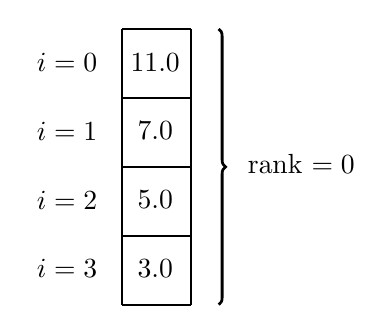
\begin{tikzpicture}[scale=3.5]
  \pgfmathsetmacro\fourth{1.0/4.0}
  \pgfmathsetmacro\xoff{0.12}
  \pgfmathsetmacro\yoff{0.12}
  \draw[xstep=\fourth,ystep=\fourth,black,thick] (0.0,0.0) grid (\fourth,1.0);
  \node at (-0.2,1.0-\yoff) {$i=0$};
  \node at (\xoff,1.0-\yoff) {$11.0$};
  \node at (-0.2,0.75-\yoff) {$i=1$};
  \node at (\xoff,0.75-\yoff) {$7.0$};
  \node at (-0.2,0.5-\yoff) {$i=2$};
  \node at (\xoff,0.5-\yoff) {$5.0$};
  \node at (-0.2,0.25-\yoff) {$i=3$};
  \node at (\xoff,0.25-\yoff) {$3.0$};
  \draw[decoration={brace,mirror,raise=5pt},decorate,line width=1pt] (0.3,0.0) -- (0.3,1.0);
  \node at (0.65,0.51) {rank $=0$};
\end{tikzpicture}


\caption{A sequential \pVec layout, all on rank $=0$ process.}
\label{fig:seqveclayout}
\end{marginfigure}

The reader is allowed to think of a \PETSc \pVec as a one-dimensional C array with its contents split across the processes in the MPI communicator.  For example, if the above code appears in \texttt{mycode.c}, and if it is run sequentially on one process, i.e.~as
\begin{cline}
$ ./mycode.c
\end{cline}
%$
then, at the end of the above create-set-assemble sequence, the storage of \texttt{x} looks like Figure \ref{fig:seqveclayout}.  However, if run as
\begin{cline}
$ mpiexec -n 2 ./mycode.c
\end{cline}
%$
then the layout looks like Figure \ref{fig:mpitwoveclayout}.  In this case the argument \texttt{PETSC\_DECIDE} in \texttt{VecSetSizes()} is active, and \PETSc's decision will be to put the first two entries of \texttt{x} on the rank $0$ process and the other two on the rank $1$ process. 

\begin{marginfigure}
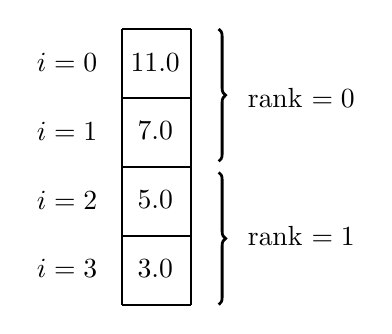
\begin{tikzpicture}[scale=3.5]
  \pgfmathsetmacro\fourth{1.0/4.0}
  \pgfmathsetmacro\xoff{0.12}
  \pgfmathsetmacro\yoff{0.12}
  \draw[xstep=\fourth,ystep=\fourth,black,thick] (0.0,0.0) grid (\fourth,1.0);
  \node at (-0.2,1.0-\yoff) {$i=0$};
  \node at (\xoff,1.0-\yoff) {$11.0$};
  \node at (-0.2,0.75-\yoff) {$i=1$};
  \node at (\xoff,0.75-\yoff) {$7.0$};
  \node at (-0.2,0.5-\yoff) {$i=2$};
  \node at (\xoff,0.5-\yoff) {$5.0$};
  \node at (-0.2,0.25-\yoff) {$i=3$};
  \node at (\xoff,0.25-\yoff) {$3.0$};
  \draw[decoration={brace,mirror,raise=5pt},decorate,line width=1pt] (0.3,0.52) -- (0.3,1.0);
  \node at (0.65,0.752) {rank $=0$};
  \draw[decoration={brace,mirror,raise=5pt},decorate,line width=1pt] (0.3,0.0) -- (0.3,0.48);
  \node at (0.65,0.251) {rank $=1$};
\end{tikzpicture}


\caption{A parallel \pVec layout on two processes.  Because we call ``\texttt{VecSetSizes(x,PETSC\_DECIDE,4)}'', \PETSc decides to split the storage in the middle.}
\label{fig:mpitwoveclayout}
\end{marginfigure}

The operation of setting values in \texttt{x} may require communication between processes, however, because entries which are to be stored on one process could be set by another process.  Such communication occurs between the \texttt{VecAssemblyBegin()} and \texttt{VecAssemblyEnd()} commands.
  
\PETSc \pMat objects are comparable to \pVecs, but they are not merely 2D C arrays even in serial (i.e.~in one-process runs).  Compared to \pVecs they require additional choices regarding parallel distribution and storage formats.  Though this is hidden inside the implementation of \pMat, the most common storage format is \emph{parallel compressed sparse row storage}, what \PETSc calls the \texttt{MATMPIAIJ} type.  In this type a range of rows is owned by each process (parallel row storage).  Within each owned range of rows only the specifically-allocated entries are stored (sparse), and these nonzero entries are stored contiguously in memory using an additional index array (compressed).  An example is shown in Figure \ref{fig:mpitwomatlayout}.

The ``specifically-allocated'' entries are generally the nonzero entries, but they are always referred-to as ``nonzero entries'' in sparse representations even though they occasionally have zero values.  Depending on how the \PETSc API is used the blanks in Figure \ref{fig:mpitwomatlayout} could be allocated memory, with value $0.0$, or unallocated.  We show these two possibilities below.

\begin{marginfigure}
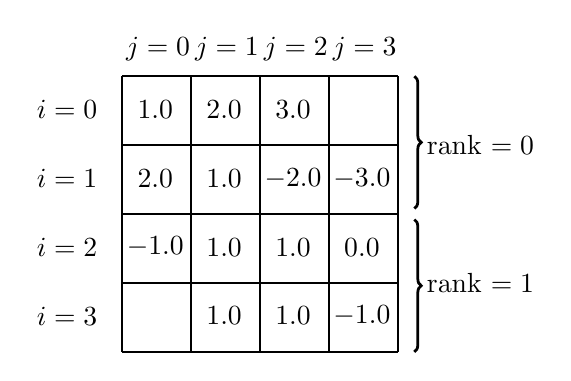
\begin{tikzpicture}[scale=3.5]
  \pgfmathsetmacro\fourth{1.0/4.0}
  \pgfmathsetmacro\xoff{0.12}
  \pgfmathsetmacro\yoff{0.12}
  \draw[xstep=\fourth,ystep=\fourth,black,thick] (0.0,0.0) grid (1.0,1.0);

  \node at (-0.2, 1.0-\yoff) {$i=0$};
  \node at (-0.2,0.75-\yoff) {$i=1$};
  \node at (-0.2, 0.5-\yoff) {$i=2$};
  \node at (-0.2,0.25-\yoff) {$i=3$};

  \node at ( 1.0-\xoff, 1.1) {$j=3$};
  \node at (0.75-\xoff, 1.1) {$j=2$};
  \node at ( 0.5-\xoff, 1.1) {$j=1$};
  \node at (0.25-\xoff, 1.1) {$j=0$};

  \node at (\xoff,1.0-\yoff) {$1.0$};
  \node at (0.25+\xoff,1.0-\yoff) {$2.0$};
  \node at (0.5+\xoff,1.0-\yoff) {$3.0$};
  \node at (0.75+\xoff,1.0-\yoff) {};

  \node at (\xoff,0.75-\yoff) {$2.0$};
  \node at (0.25+\xoff,0.75-\yoff) {$1.0$};
  \node at (0.5+\xoff,0.75-\yoff) {$-2.0$};
  \node at (0.75+\xoff,0.75-\yoff) {$-3.0$};

  \node at (\xoff,0.5-\yoff) {$-1.0$};
  \node at (0.25+\xoff,0.5-\yoff) {$1.0$};
  \node at (0.5+\xoff,0.5-\yoff) {$1.0$};
  \node at (0.75+\xoff,0.5-\yoff) {$0.0$};

  \node at (\xoff,0.25-\yoff) {};
  \node at (0.25+\xoff,0.25-\yoff) {$1.0$};
  \node at (0.5+\xoff,0.25-\yoff) {$1.0$};
  \node at (0.75+\xoff,0.25-\yoff) {$-1.0$};

  \draw[decoration={brace,mirror,raise=5pt},decorate,line width=1pt] (1.01,0.52) -- (1.01,1.0);
  \node at (1.3,0.752) {rank $=0$};
  \draw[decoration={brace,mirror,raise=5pt},decorate,line width=1pt] (1.01,0.0) -- (1.01,0.48);
  \node at (1.3,0.251) {rank $=1$};
\end{tikzpicture}


\caption{A parallel \pMat layout, on two processes, of a $4\times 4$ matrix with 13 nonzero entries.}
\label{fig:mpitwomatlayout}
\end{marginfigure}

\pMat objects are linear operators and their ``purpose'' is to act on (multiply) \pVecs.  Of course, the result \pVec from a \pMat-\pVec product is a linear combination of the columns of the \pMat \citep{TrefethenBau1997}.  Thus, in practice and by default, parallel row storage of the \pMat means these things:
\begin{itemize}
\item \PETSc internally distributes the rows of the \pMat $A$ the same way as the entries of the intended \emph{output} (i.e.~column) \pVec.  Thus if $A\bx=\bb$ for some \pVec $\bx$ then row $i$ of $A$ is on the rank $m$ MPI process if and only if entry $i$ of \pVec $\bb$ is on the rank $m$ process.\sidenote{This is the outcome when \texttt{PETSC\_DECIDE} is used in setting both the \pVec and \pMat sizes and they have the same number of rows.}
\item As \PETSc computes the \pMat-\pVec product, it communicates (``scatters'' using MPI calls) the needed portions of the \pVec to the processes.
\item After the scatter the \pMat-\pVec product is a local operation, requiring no further communication.
\end{itemize}


\section{Example \pMat assembly}

One doesn't really need to know how \PETSc works internally in order to assemble a matrix.  For example, here is one straightforward way to fill a $4\times 4$ matrix, the one shown in Figure \ref{fig:mpitwomatlayout}, one row at a time by using a \texttt{for} loop over the row index \texttt{i}:
\begin{code}
Mat    A;
int    i, j[4] = {0, 1, 2, 3};
double aA[4][4] = {{ 1.0,  2.0,  3.0,  0.0},
                   { 2.0,  1.0, -2.0, -3.0},
                   {-1.0,  1.0,  1.0,  0.0},
                   { 0.0,  1.0,  1.0, -1.0}};

MatCreate(PETSC_COMM_WORLD,&A);
MatSetSizes(A,PETSC_DECIDE,PETSC_DECIDE,4,4);
MatSetFromOptions(A);
MatSetUp(A);
for (i=0; i<4; i++) {
    MatSetValues(A,1,&i,4,j,aA[i],INSERT_VALUES);
}
MatAssemblyBegin(A,MAT_FINAL_ASSEMBLY);
MatAssemblyEnd(A,MAT_FINAL_ASSEMBLY);
\end{code}

The function \texttt{MatSetValues()} sets multiple entries in a \pMat as long as they \emph{form a block}, in this case a row which is a $1\times 4$ block.  (Generally a ``block'' means a product of a list of row indicies and a list of column indices.)  The ``\texttt{1,\&i}'' arguments indicate that we are setting one row index \texttt{i}.  The ``\texttt{4,j}'' arguments indicate that integer array \texttt{j} has the 4 column indices for the entire row.  Note that ``\texttt{aA[i]}'' is a C \emph{pointer}, essentially of type \texttt{double*}, to the $i$th row of $A$.

Assembly one row at a time is common in PDE-type applications, where a row represents the discrete version of the PDE at a grid/mesh location.  In such cases there may be only a few nonzero entries per row.

However, the example above treats the matrix as dense: every entry is filled including those with value $0.0$.  The same matrix could be formed by inserting only the 13 nonzero entries, which is the usage pattern would expect for a sparse matrix.  In the current case this is mildly awkward because \texttt{MatSetValues()} is designed to set a \emph{block} of entries, as already noted.  Here we break up $A$ into three contiguous blocks of nonzeros: we call \texttt{MatSetValues()} on a $3\times 3$ block, then on a $1\times 3$ block, and then we call \texttt{MatSetValue()} on a single entry.  This example illustrates the general block-wise procedure of assembly, and the \texttt{for} loop is gone, but one cannot call it elegant:
\begin{code}
int    i1[3] = {0, 1, 2},
       j1[3] = {0, 1, 2},
       i2 = 3,
       j2[3] = {1, 2, 3},
       i3 = 1,
       j3 = 3;
double aA1[9] = { 1.0,  2.0,  3.0,
                  2.0,  1.0, -2.0,
                 -1.0,  1.0,  1.0},
       aA2[3] = { 1.0,  1.0, -1.0},
       aA3 = -3.0;
...
MatSetValues(A,3,i1,3,j1,aA1,INSERT_VALUES);
MatSetValues(A,1,&i2,3,j2,aA2,INSERT_VALUES);
MatSetValue(A,i3,j3,aA3,INSERT_VALUES);
...
\end{code}
Exercise \ref{chap:ls}.\ref{exer:ls:sparseinsertion} asks you to confirm that the solution to the corresponding linear system is the same.  \label{page:ls:sparseinsertion}

\PETSc can show us the entries in the \pMat in different formats at runtime.  Assuming the \pMat was assembled using the second (sparse) method above, and that the above lines appeared in \texttt{mycode.c}, then:
\begin{cline}
$ ./mycode -mat_view
Mat Object: 1 MPI processes
  type: seqaij
row 0: (0, 1.)  (1, 2.)  (2, 3.) 
row 1: (0, 2.)  (1, 1.)  (2, -2.)  (3, -3.) 
row 2: (0, -1.)  (1, 1.)  (2, 1.) 
row 3: (1, 1.)  (2, 1.)  (3, -1.) 
$ ./mycode -mat_view ::ascii_dense
Mat Object: 1 MPI processes
  type: seqaij
 1.00000e+00  2.00000e+00  3.00000e+00  0.00000e+00
 2.00000e+00  1.00000e+00  -2.00000e+00  -3.00000e+00
 -1.00000e+00  1.00000e+00  1.00000e+00  0.00000e+00
 0.00000e+00  1.00000e+00  1.00000e+00  -1.00000e+00
\end{cline}
The first view shows the sparse storage format, with values as pairs with column index and value.  The second view is ``dense'': all zero values are shown, whether allocated or not.

The output from option \texttt{-mat\_view} occurs at the completion of the \texttt{MatAssemblyBegin/End()} calls.  The following examples illustrate more possibilities for viewing a \pMat, using the up-to-three-argument option form:\begin{itemize}
\item show the sparsity pattern graphically using the X window system
\begin{codeplain}
-mat_view draw -draw_pause 1
\end{codeplain}
\item save to file \texttt{mat.dat} in \PETSc's scalable binary format
\begin{codeplain}
-mat_view binary:mat.dat
\end{codeplain}
\item save to text file \texttt{mat.m} in Matlab text format
\begin{codeplain}
-mat_view ascii:mat.m:ascii_matlab
\end{codeplain}
\item print at \texttt{stdout} in Matlab text format
\begin{codeplain}
-mat_view ::ascii_matlab
\end{codeplain}
\end{itemize}
In the last form, and in the \texttt{ascii\_dense} case earlier, the first two positional arguments are not needed because the default format is \texttt{ascii} and because \texttt{stdout} is used if there is no file name.  However, the last argument (\texttt{ascii\_dense} or \texttt{ascii\_matlab}, respectively, in these two cases) must be put in the third position by starting with two colons.

In the cases shown above the matrix was stored in serial compressed sparse row format, the \texttt{MATSEQAIJ} type, because of the one-process run.  If the code is run in parallel, i.e.~by \texttt{ mpiexec -n N ./mycode }, then \texttt{ -mat\_view }  reports \texttt{ type:~mpiaij } corresponding to \pMat type \texttt{MATMPIAIJ}, the ``parallel compressed sparse row storage'' described above.


\section{A small linear system}

We now know how to create, fill, and destroy \pVec and \pMat objects.  Code \ref{code:vecmatksp} shows \texttt{vecmatksp.c} which does these steps for the linear system
\begin{equation}
\begin{bmatrix} 1 & 2 & 3 & 0 \\
                2 & 1 &-2 &-3 \\
               -1 & 1 & 1 & 0 \\
                0 & 1 & 1 &-1 \end{bmatrix}
\begin{bmatrix} x_0 \\ x_1 \\ x_2 \\ x_3 \end{bmatrix}
=
\begin{bmatrix} 7 \\ 1 \\ 1 \\ 3 \end{bmatrix}.
\end{equation}

A \pKSP object solves the linear system, with the specific solution algorithm only chosen at runtime.  It has the expected \texttt{Create/SetFromOptions/Destroy} sequence.  In addition, at the set-up stage for the linear system we tell the \pKSP about the matrix via the command
\begin{code}
KSPSetOperators(ksp,A,A);
\end{code}

Why do we list \texttt{A} twice in calling \texttt{KSPSetOperators()}?  The reason is that at runtime we generally choose a preconditioning method which builds $M^{-1}$ in equation \eqref{introleftpre} or \eqref{introrightpre} from $A$ or from an approximation of $A$.  For example, \emph{incomplete LU} factorization of $A$ (``ILU($0$)'') can be used in generating $M^{-1}$.  Alternatively, $M$ could be the diagonal of $A$ as in the example on page \pageref{example:ls:jacobirichardson}.  The second matrix argument to \texttt{KSPSetOperators()} is this \pMat from which $M^{-1}$ is built.

\cinput{vecmatksp.c}{\CODELOC}{Solve a small linear system.}{//START}{//END}{code:vecmatksp}

Note that we do not supply $M$ \emph{itself} because that would obstruct easy choice among preconditioners at runtime, and require the user to write extra code.  Instead we supply ``material'' from which the preconditioning action $M^{-1}$ is built.  The most common such material is $A$ itself, as here.  In Jacobi preconditioning, for example, \PETSc extracts the diagonal from the ``material.''  Or it computes ILU($0$) factors $L$ and $U$ from $A$, in which case $A \approx LU$ is only an approximation, but $M^{-1} = (LU)^{-1} = U^{-1} L^{-1}$ may be a helpful preconditioner.

To actually solve the system we call
\begin{code}
KSPSolve(ksp,b,x);
\end{code}
This supplies the right-hand side of the system, an allocated and assembled \pVec \texttt{b}, and space for the solution, an allocated \pVec \texttt{x}.  After this we display the solution using \texttt{VecView()}.  Everything else about Code \ref{code:vecmatksp} should be self-explanatory.

Let us compile and run it:
\begin{cline}
$ cd c/ch2/
$ make vecmatksp
...
$ ./vecmatksp
Vec Object: 1 MPI processes
  type: seq
1
0
2
-1
\end{cline}
%$
The reader can even check the correctness of this solution by hand.


\section{Revealing solvers at runtime}

To see more of what happened when we ran \texttt{vecmatksp.c} above, we could start by viewing the \pVec and \pMat objects.  But the result of
\begin{cline}
$ ./vecmatksp -vec_view -mat_view
\end{cline}
%$
is completely as expected, and thus not shown.  This output tells us nothing about the solution process, nor does it give any hints on alternative ways of solving the equations.

Here is a key idea which cannot be over-emphasized:
\begin{quote}
\emph{learning \PETSc requires viewing \emph{solver} objects at runtime.}
\end{quote}
So we use \texttt{-ksp\_view}; the output is slightly-clipped for clarity:
\begin{cline}
$ ./vecmatksp -ksp_view
KSP Object: 1 MPI processes
  type: gmres
    GMRES: restart=30, using Classical (unmodified) Gram-Schmidt ...
    GMRES: happy breakdown tolerance 1e-30
  maximum iterations=10000, initial guess is zero
  tolerances:  relative=1e-05, absolute=1e-50, divergence=10000
  left preconditioning
  using PRECONDITIONED norm type for convergence test
PC Object: 1 MPI processes
  type: ilu
    ILU: out-of-place factorization
    0 levels of fill
    tolerance for zero pivot 2.22045e-14
    matrix ordering: natural
    factor fill ratio given 1, needed 1
      Factored matrix follows:
        Mat Object:         1 MPI processes
          type: seqaij
          rows=4, cols=4
          package used to perform factorization: petsc
          total: nonzeros=14, allocated nonzeros=14
          ...
  linear system matrix = precond matrix:
  Mat Object:   1 MPI processes
    type: seqaij
    rows=4, cols=4
    total: nonzeros=16, allocated nonzeros=20
    ...
Vec Object: 1 MPI processes
  type: seq
1
0
2
-1
\end{cline}
%$
Here is some of what we learn:
\begin{itemize}
\item The default \pKSP solver is GMRES.  This is \texttt{-ksp\_type gmres} as a command-line option.  Also, as already noted, GMRES restarts after a number of iterations so as to limit memory usage, and the default is \texttt{-ksp\_gmres\_restart 30}.
\item The default convergence tolerances for the \pKSP are \texttt{-ksp\_rtol 1.0e-5} and \texttt{-ksp\_atol 1.0e-50}.  In particular, iterations stop when the residual norm has been reduced by $10^5$.
\item Inside every \pKSP is a \pPC preconditioner object.  We did not have to ask for one when writing the code.
\item The \pPC object has a copy of $A$ (second ``\texttt{Mat Object:}'' line), because it was supplied as the second argument to \texttt{KSPSetOperators()} above.
\item The default \pPC is left preconditioning with ILU, i.e.~incomplete LU factorization, which is \texttt{-pc\_type ilu} as a runtime option.\sidenote{We will see in a moment that this is the \emph{serial} default \pPC, and there is more going on in parallel.}  This preconditioner has ``\texttt{0 levels of fill}'', which explains the notation ``ILU($0$)'', but it is done ``\texttt{out-of-place}'' meaning that the factors occupy an additional \pMat (first ``\texttt{Mat Object:}'' line).
\end{itemize}

While option \texttt{-ksp\_view} tells us what the solver \emph{is}, option \texttt{-ksp\_monitor} shows what it \emph{does}.  In this case, the \pKSP iteration is short:
\begin{cline}
$ ./vecmatksp -ksp_monitor
  0 KSP Residual norm 2.449489742783e+00
  1 KSP Residual norm 1.520235486122e-15
Vec Object: 1 MPI processes
...
\end{cline}
%$
The reason that the residual drops to nearly zero in one iteration is that GMRES sees a preconditioned system with an identity matrix $M^{-1} A = I$ in \emph{this case}.  That is because the ILU operation on this particular $A$ is actually a full LU factorization: $M=LU=A$.  Our $A$ is allocated as a dense matrix so the exact LU factorization requires no further ``fill-in.''\sidenote{By definition, ``fill-in'' occurs in a sparse matrix \cite{TrefethenBau1997} operation in which previously un-allocated zeros are replaced by non-zeros which use up memory.}  The next example \texttt{tri.c}, and the examples in later Chapters, are more representative because they involve sparse matrices.

For a small system like this, of course, a direct solve can be chosen deliberately.  To see how to do it, first do
\begin{cline}
$ ./vecmatksp -help | grep ksp_type
  -ksp_type <gmres>: Krylov method (one of) cg ... preonly ... (KSPSetType)
\end{cline}
%$
and
\begin{cline}
$ ./vecmatksp -help | grep pc_type
  -pc_type <ilu>: Preconditioner (one of) none jacobi ... lu ... (PCSetType)
\end{cline}
%$
This shows the many Krylov solver and preconditioner options.  One of the preconditioners is ``\texttt{lu}'' for the full LU decomposition.  In this case we \emph{do not} want iterations, and one of the \pKSP options is ``\texttt{preonly}''.  Thus a direct solver combination is
\begin{cline}
$ ./vecmatksp -ksp_type preonly -pc_type lu
\end{cline}
%$
The reader should check that the output of \texttt{-ksp\_view} is as intended.

When solving on multiple MPI processes, using ILU($0$) as the default preconditioner makes no sense.  This is because, even when fill-in is avoided, the LU factorization algorithm would involve a great deal of interprocess communication.  However, there are blocks along the diagonal of the system matrix $A$ which are entirely owned by a single process.  The ILU($0$) method can be applied to these, and the result treated as an approximation $M^{-1}\approx A^{-1}$.  That is, the blocks along the diagonal can be approximately inverted by ILU($0$), and the result treated as a block-diagonal (i.e.~block-Jacobi) preconditioner.

The default \PETSc \pKSP settings \emph{in parallel} correspond to options
\begin{quote}
\texttt{-ksp\_type gmres -pc\_type bjacobi -sub\_pc\_type ilu}
\end{quote}
Namely:
\begin{itemize}
\item The default \pKSP remains GMRES with restart 30.
\item The default \pPC is \texttt{bjacobi}, i.e.~application of approximate diagonal-block inverses as $M^{-1}$.
\item Inside the \pPC is a \texttt{sub\_pc} object, also a \pPC, which is ILU($0$),\sidenote{There is even a \texttt{sub\_ksp} object, but it is \texttt{preonly}.} and this generates the approximate diagonal-block inverses.
\end{itemize}
The reader can confirm the situation by running
\begin{cline}
mpiexec -n 2 ./vecmatksp -ksp_view
\end{cline}

Surely that's enough runtime options for now.  Of course there will be more, especially in later Chapters when we solve PDEs.


\section{A sparse system of arbitrary size}

We have seen how \PETSc code sets up and solves linear systems, but there is more to say.  The next example \texttt{tri.c}, split into Codes \ref{code:tripartone} and \ref{code:triparttwo}, introduces the following additional concepts and associated function calls:
\begin{itemize}
\item Creating an integer option by \texttt{PetscOptionsXXX()} calls, so that the size of the linear system can be controlled at runtime.
\item Using \texttt{VecDuplicate()} for allocation.
\item Assembling a system of arbitrary size across an arbitrary number of processes, using \texttt{MatGetOwnershipRange()} to only set locally-owned rows.
\item Using \texttt{VecAXPY()}, \texttt{VecNorm()}, and \texttt{PetscPrintf()} to compute and display the numerical error in a case where the exact solution is known.
\end{itemize}

Build and run the code:
\begin{cline}
$ make tri
$ ./tri -ksp_monitor -a_mat_view ::ascii_dense
Mat Object:(a_) 1 MPI processes
  type: seqaij
  3.00000e+00  -1.00000e+00   0.00000e+00   0.00000e+00 
 -1.00000e+00   3.00000e+00  -1.00000e+00   0.00000e+00 
  0.00000e+00  -1.00000e+00   3.00000e+00  -1.00000e+00 
  0.00000e+00   0.00000e+00  -1.00000e+00   3.00000e+00 
  0 KSP Residual norm 3.302822756884e+00 
  1 KSP Residual norm 5.519370044893e-16 
error for m = 4 system is |x-xexact|_2 = 5.1e-16
\end{cline}

\cinputpart{tri.c}{\CODELOC}{Set up \pVec and \pMat objects for a tridiagonal system.}{I}{//STARTSETUP}{//ENDSETUP}{code:tripartone}

The first new tool used in Code \ref{code:tripartone} is bracketed by \texttt{PetscOptionsBegin()} and \texttt{PetscOptionsEnd()}, namely the call to \texttt{PetscOptionsInt()}.  The \texttt{Begin} method sets a prefix ``\texttt{-tri\_...}'' so that the new option we create is distinguished from the many built-in \PETSc options that start with \texttt{-ksp\_...} or \texttt{-vec\_...} or whatever.  Here \texttt{PetscOptionsInt()} creates option \texttt{-tri\_m} so the user can set the variable \texttt{m}, and leave the default \texttt{m}$=4$ unaltered if the option is not set.

To see the option and its default value in \texttt{-help} output do
\begin{cline}
$ ./tri -help | grep tri_
Solve a tridiagonal system of arbitrary size.  Option prefix = tri_.
  -tri_m <4>: dimension of linear system (None)
\end{cline}
%$
Here, for instance, we reset the system size to be small:
\begin{cline}
$ ./tri -tri_m 2
error for m = 2 system is |x-xexact|_2 = 8.0e-16
\end{cline}
%$

\cinputpart{tri.c}{\CODELOC}{Assemble and solve.}{II}{//ENDSETUP}{//ENDSOLVE}{code:triparttwo}

After setting up the new option, next in \texttt{tri.c} the numerical solution \pVec \texttt{x} is created just as we did in the last example \texttt{vecmatksp.c} (Code \ref{code:vecmatksp}).  But now we also want to create \pVecs \texttt{b} and \texttt{xexact}; the former is the right-hand side of the linear system and the latter holds the exact solution to the linear system so that we can evaluate the error in the numerical solution.  Though at this stage we have not filled any entries of \texttt{x}, we can save repetitive function calls to \texttt{VecCreate/SetSizes/SetFromOptions()}, when creating these additional \pVecs, by calling \texttt{VecDuplicate()} to allocate \pVecs just like \texttt{x}.  (There is a different method for copying the contents of \pVecs, namely \texttt{VecCopy()}.  It requires that the two \pVecs are already allocated and have the same layout.)

Next we assemble the matrix $A$.  This is a boring tridiagonal matrix with $3$ on the diagonal and $-1$ in the super- and sub-diagonals.  Though boring, we want to assemble it efficiently in parallel, something that will be important when solving 2D and 3D PDEs in later chapters.  However, only when \texttt{tri.c} is run do we know how many processes are in use.  The method \texttt{MatGetOwnershipRange()} tells our program, running on a particular process (rank), what rows it owns locally.  In the case of a many structured matrices like this one, we can avoid all interprocess communication by assembling exactly the rows we own.  As seen at the top of Code \ref{code:triparttwo}, we call
\begin{quote}
\texttt{MatGetOwnershipRange(A,\&Istart,\&Iend)}
\end{quote}
to obtain the starting and ending row indices for the local process.  These are used as limits in a \texttt{for} loop over the locally own rows.  We use \texttt{MatSetValues()} to actually set the entries of $A$ and \texttt{MatAssemblyBegin/End()} to complete the assembly of $A$.

We need to assemble the right-hand side $\bb$ of the linear system and also the exact solution $\bx_{\text{exact}}$ to the linear system ($A\bx_{\text{exact}} = \bb$).  The easiest way, for demonstration purposes here, is to \emph{choose} $\bx_{\text{exact}}$ and then compute $\bb$ by multiplying by $A$.  Thus, we set (unimportant) values for \texttt{xexact}, and call \texttt{VecAssemblyBegin/End()} on it.  Then we compute \texttt{b} by calling \texttt{MatMult(A,xexact,b)}.

As in \texttt{vecmatksp.c} we set up  the \pKSP and then call \texttt{KSPSolve()} to approximately solve $A\bx = \bb$.  Option \texttt{-ksp\_monitor} prints the residual norm $\|\bb-A\bx_k\|_2$ at runtime.  In this case we also want to see that the actual error
	$$\|\bx - \bx_{\text{exact}}\|_2$$
is small when the \pKSP completes its work.  So, after getting \texttt{x} from \texttt{KSPSolve()} we compute the error with two commands,

\medskip
\begin{tabular}{lcrcl}
\text{\texttt{VecAXPY(x,-1.0,xexact)}}       & : & $\bx$                   & $\leftarrow$ & $-1\, \bx_{\text{exact}} + \bx$ \\
\text{\texttt{VecNorm(x,NORM\_2,\&errnorm)}} & : & \text{\texttt{errnorm}} & $\leftarrow$ & $\|\bx\|_2$.
\end{tabular}

\medskip
\noindent and then print \texttt{errnorm} by calling \texttt{PetscPrintf()}.


\section{A first look at performance}

The linear system assembled by \texttt{tri.c} is about as easy to solve as they get.   It is tridiagonal, symmetric, diagonally-dominant, and positive definite.\sidenote{See Exercise \ref{chap:ls}.\ref{exer:computeeigs}.}  So \PETSc ought to be able to solve it quickly, almost all Krylov methods should apply, and parallelization ought to be effective.

\newcommand{\WORKSTATION}{\textsc{workstation}\xspace}
We can time a one-process solution:
\begin{cline}
$ time ./tri -tri_m 10000
error for m = 10000 system is |x-xexact|_2 = 8.0e-13
real 0.04
user 0.04
sys 0.00
\end{cline}
%$
\label{defineworkstation}
These times were taken on the author's 2012-era workstation with 16 GB memory and a single Intel Core i7-3820 4-core CPU running at 3.60GHz.  From now on we call this machine \WORKSTATION.

Only the ``\texttt{real}'' time above is worth considering.  From now on we will use an alias to get just this time:
\begin{cline}
$ alias timer='time -f "real %e"'
\end{cline}
%$

The above timing result of $.04$ seconds suggests that this $m=10^4$ dimension system is not yet big enough to be worth testing, so we experiment on what $m$ gives a linear system with noticeable solution time.  Here is a roll-your-own Bash loop to time some bigger systems:
\begin{cline}
$ export SIZES="10000 100000 1000000 10000000"
$ for M in $SIZES; do timer ./tri -tri_m $M; done
error for m = 10000 system is |x-xexact|_2 = 8.0e-13
real 0.01
error for m = 100000 system is |x-xexact|_2 = 3.1e-12
real 0.07
error for m = 1000000 system is |x-xexact|_2 = 4.8e-11
real 0.32
error for m = 10000000 system is |x-xexact|_2 = 3.5e-10
real 2.39
\end{cline}
We see that the default \PETSc \pKSP and \pPC methods\sidenote{GMRES with ILU($0$) preconditioning.} solve a system of size $m=10^7$ (ten million) in a time of a few seconds on \WORKSTATION.

Will other methods and/or more processors speed up the solution of a linear system of this size?  We can try a direct solver (\texttt{-ksp\_type preonly -pc\_type lu}), the default serial solver (\texttt{-ksp\_type gmres -pc\_type ilu}), or the default parallel solver (\texttt{-ksp\_type gmres -pc\_type bjacobi -sub\_pc\_type ilu}).  We can turn off preconditioning (\texttt{-pc\_type none}) or switch from ILU($0$)-based preconditioning to Jacobi preconditioning (\texttt{-pc\_type jacobi}).  In fact, to generate Table \ref{tab:tritiming} below we did 16 runs like this:
\begin{cline}
$ timer mpiexec -n N ./tri -tri_m 20000000 -ksp_rtol 1.0e-10 -ksp_type KSP -pc_type PC
\end{cline}
%$
for $N=1$ and $N=4$, and several \pKSP/\pPC choices.  The tighter tolerance \texttt{-ksp\_rtol 1.0e-10} was added because a fair comparison of iterative and direct methods needs significant accuracy in the iterative ones.

\newcommand{\intime}[1]{\input{timing/tri/#1}}
\begin{table}
\texttt{
\begin{tabular}{llll}
\underline{KSP}\hspace{0.5in} & \underline{PC}\hspace{0.8in} & \underline{N=1 \textrm{time (s)}}\hspace{0.3in} & \underline{N=4 \textrm{time (s)}} \\
preonly    & lu          & \intime{preonly.lu.1}       &  \\
           & cholesky    & \intime{preonly.cholesky.1} &  \\
richardson & jacobi      & \intime{richardson.jacobi.1}& \intime{richardson.jacobi.4} \\
gmres      & none        & \intime{gmres.none.1}       & \intime{gmres.none.4} \\
           & jacobi      & \intime{gmres.jacobi.1}     & \intime{gmres.jacobi.4} \\
           & ilu         & \intime{gmres.ilu.1}        &  \\
           & bjacobi+ilu &                             & \intime{gmres.bjacobi.4} \\
cg         & none        & \intime{cg.none.1}          & \intime{cg.none.4} \\
           & jacobi      & \intime{cg.jacobi.1}        & \intime{cg.jacobi.4} \\
           & icc         & \intime{cg.icc.1}           &  \\
           & bjacobi+icc &                             & \intime{cg.bjacobi.4} \\
\end{tabular}
}
\caption{Times for \texttt{tri.c} to solve systems of dimension $m=2\times 10^7$.  In this case the matrix is \emph{tridiagonal}, \emph{symmetric}, \emph{diagonally-dominant}, and \emph{positive definite}.  All runs were on \WORKSTATION (see page \pageref{defineworkstation}).} \label{tab:tritiming}
\end{table}

This Table deserves discussion:
\begin{itemize}
\item Entries ``\texttt{bjacobi+ilu}'' and ``\texttt{bjacobi+icc}'' correspond to options \texttt{-pc\_type bjacobi -sub\_pc\_type ilu} and \texttt{-pc\_type bjacobi -sub\_pc\_type icc}, respectively.  As already noted, the first of these is the parallel default, and the Table suggests why this is.

\item Counting floating point operations shows the leading-order work for Cholesky is $m^3/3$ while for LU it is $2 m^3/3$ \citep{TrefethenBau1997}.  This is reflected in the direct-solve results using \texttt{-ksp\_type preonly}.

\item A diagonally-dominant tridiagonal problem is very well-behaved for direct methods because no fill-in or pivoting occurs when they are applied, but the reader should not assume that generic $N=10^7$ dimension systems are good candidates for direct solves.

\item CG and Cholesky methods, namely \pKSP method \texttt{cg} and \pPC methods \texttt{cholesky} or \texttt{icc} (incomplete-Cholesky), respectively, apply to symmetric positive-definite matrices only.  We see some benefit to using CG on one-process runs, compared to the general (non-symmetric) method GMRES, but the matrix here is so well-behaved that exploiting symmetry gives no noticable benefit.

\item There is some speed-up from $N=1$ to $N=4$ processes on this single node 4-core \WORKSTATION.  The two (or slightly more) times speed-up is relatively uniform across methods.  But apparently using four cores does not guarantee anywhere near four-times speed-up.
\end{itemize}

In future Chapters, ``real'' linear and non-linear systems will be generated by discretizing PDEs.  Then we will create timing tables like Table \ref{tab:tritiming}, and re-consider the results.

\begin{marginfigure}
\bigskip
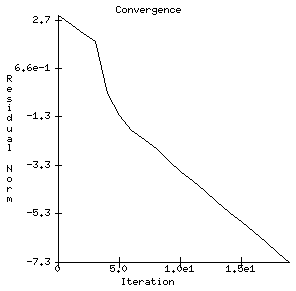
\includegraphics[width=0.9\textwidth]{figs/line-graph-tri}
\caption{\PETSc can use X windows to produce line graphs at run time.  (This is not to say they are pretty.)}
\label{fig:line-graph-tri}
\end{marginfigure}

It is worth noting at this point that \PETSc can generate graphics showing convergence of the above iterative (Krylov) methods, at least if \PETSc was built with X Window System support.  The line graph in Figure \ref{fig:line-graph-tri}, from
\begin{cline}
$ ./tri -tri_m 1000000 -ksp_rtol 1.0e-10 -pc_type jacobi \
    -ksp_monitor_lg_residualnorm -draw_pause 1
\end{cline}
%$
shows the residual norm logarithm versus the iteration number.


\section{Parallel preconditioning}

There is one more ``fact of life'' to point out, again relating to numerical linear algebra.  We can demonstrate it using \texttt{tri.c} runs:
\begin{cline}
$ mpiexec -n N ./tri -tri_m 100 -ksp_type cg -pc_type bjacobi \
    -sub_pc_type icc -ksp_converged_reason
\end{cline}
%$
Compare $N=2$ and $N=20$.  We get convergence to the default tolerance in $3$ and $5$ iterations, respectively, and the final reported numerical error is quite different in the two cases.

In general, we observe there is a

\begin{enumerate}
\setcounter{enumi}{3}
\item \emph{Most preconditioning methods have a process-count dependence.}  Preconditioning schemes, including block-Jacobi and Schwarz methods (Chapter \ref{chap:pr}), act differently depending on the number of MPI processes.
\end{enumerate}

\noindent Note that this process-count dependence has a stronger influence on final answers than the other parallel ``fact of life'', namely that parallel reductions are not deterministic (Chapter \ref{chap:gs}).

The difference does not arise in the Krylov iteration implementation.  Rather, the preconditioning matrices $M^{-1}$ applied at each Krylov iteration are actually different matrices in the $N=2$ and $N=20$ cases.  In particular, on $N$ processes the block-Jacobi matrix is
\begin{equation}
  M^{-1} = \begin{bmatrix}
           M_0^{-1} & & & \\
           & M_1^{-1} & & \\
           & & \ddots & \\
           & & & M_{N-1}^{-1}
           \end{bmatrix}   \label{eq:ls:parallelpreconditioner}
\end{equation}
where each block $M_i$ is the product of the \texttt{icc} factors acting on those rows which are owned on the rank $i$ process.  For any nontrivial preconditioner, even one based on diagonal blocks of a tridiagonal matrix as here, different sets of rows ``communicate'' at the preconditioning stage depending on the process count.

What if you do not want this dependence?  On the one hand, you can make the reported numerical error nearly process-count-independent by asking that it be small (e.g.~\texttt{-ksp\_rtol 1.0e-14}), but then the difference in iteration count is even stronger ($3$ and $13$ iterations on $N=2$ and $N=20$ processes, respectively).  On the other hand, if you replace ``\texttt{-pc\_type bjacobi -sub\_pc\_type icc}'' with ``\texttt{-pc\_type none}'' or ``\texttt{-pc\_type jacobi}'' then runs on $N=2$ and $N=20$ processes all get identical numerical error results after 12 iterations.\sidenote{I.e.~all four runs show the same numerical error and iteration count.}  These preconditioners do not communicate any information between rows at all, and thus they exhibit no dependence.  However, \emph{good} preconditioners, as we will see, cannot be that trivial.

Fundamentally, preconditioning is useful if can both be applied quickly \emph{and} it has a desirable effect on the spectrum of the matrix.\sidenote{``Desirable'' is relative to the Krylov solver in use.}  Quick parallel application requires avoiding interprocess communication, but desirable spectral effect generally requires using multi-row information, at least from multiple rows owned by the process.  We will not fight against this situation, but we must be careful to evaluate parallel preconditioner effectiveness by measuring execution time, or execution time per degree of freedom, for example, and not only by counting Krylov iterations.


\bigskip
\section{Exercises}

\renewcommand{\labelenumi}{\arabic{chapter}.\arabic{enumi}\quad}
\begin{enumerate}
\item \label{exer:ls:jacobirichardson}  Suppose a square matrix $A$ with nonzero diagonal entries is decomposed into diagonal and lower/upper triangular parts as $A=D+L+U$.  Show that the Jacobi iteration $\bu_{k+1} = D^{-1} \left(\bb - L \bu_k - U \bu_k\right)$ is the same as the $\omega=1$ Richardson iteration \eqref{introrichardson} applied to the left-preconditioned system \eqref{introleftpre} with $M=D$.  Formulate and prove a corresponding statement about the Gauss-Seidel iteration $\bu_{k+1} = (D+L)^{-1} \left(\bb - U \bu_k\right)$.
\item \label{exer:ls:showconvergethm}  Show \eqref{introconvergethm}.

\item \label{exer:ls:errornorms}  Show \eqref{relativenormbounds}.
%For the left inequality, note first that $\|\br_0\| = \|\bb - A \bu_0\| \le \|A\| \|A^{-1} \bb - \bu\| = \|A\| \|\be_0\|$, and second that $\|\bu\| = \|A^{-1}\bb\| \le \|A^{-1}\| \|\bb\|$ so $1 / \|\bb\| \le \|A\| / \|\bu\|$.  Combining these gives the left inequality.

\item On page \pageref{eq:ls:krylovgoal} we note that a Krylov space approximation $p_{n-1}(A)\bb$ to the solution $A^{-1}\bb$ is close if $p_{n-1}(z)$ is close to $1/z$ on the spectrum of $A$.  Prove this for invertible diagonalizable matrices $A=S\Lambda S^{-1}$, with $\Lambda$ diagonal, by showing
	$$\|p_{n-1}(A) - A^{-1}\| \le \,\kappa(S)\, \max_{\lambda \in \sigma(A)} |p_{n-1}(\lambda) - \lambda^{-1}|$$
where $\kappa(S) = \|S\| \|S^{-1}\|$ is the condition number.\sidenote{Here $\|\cdot\|$ is any induced matrix norm.  However, if $A$ is \emph{normal} then $S$ can be chosen to be unitary, in which case $\kappa(S)=1$ in the $2$-norm.}

\item For the $\omega=1$ Richardson iteration \eqref{introrichardson} and $\bu_0=\bb$ we obtain $\bu_k = q_k(A) \bb$ for polynomials $q_k$ given by \eqref{richpolys}.  Show that if $\lim_{k\to\infty} q_k=q_\infty$ exists then $q_\infty(x)=1/x$.  On the other hand, by setting $y=1-x$ and defining $Q_k(y)=q_k(1-y)$, show $Q_k(y)$ is the partial sum of a well-known series with a well-known radius of convergence.

\item \label{exer:ls:sparseinsertion}  Modify \texttt{vecmatksp.c} to a new program \texttt{vmksparse.c} which uses the sparse insertion method shown on page \pageref{page:ls:sparseinsertion}.  Confirm that the result is the same for the solution of the linear system, but note how the \texttt{-mat\_view} results from the two programs differ.

\item \label{exer:ls:rankzerosetsall}  In the text describing \texttt{vecmatksp.c} we assert that communication might occur during the \texttt{VecAssemblyBegin/End()} calls.  However, as \texttt{vecmatksp.c} is written, each process has all the values it needs.\sidenote{Thus the \texttt{VecAssemblyBegin/End()} calls actually have the effect of ignoring all set values except those that go on the current process.}  To demonstrate a case where communication occurs, modify \texttt{vecmatksp.c} to a new program \texttt{vmkrankzero.c} by adding
\begin{codeplain}
MPI_Comm_rank(PETSC_COMM_WORLD,&rank)
\end{codeplain}
as in \texttt{e.c} in Chapter \ref{chap:gs}.  Then surround the \texttt{VecSetValues(b,\dots)} and \texttt{MatSetValues(A,\dots)} lines in \texttt{vecmatksp.c} with conditional ``\verb|if (rank == 0) { ... }|'' so that \texttt{...SetValues()} is only called from one process, even in parallel.  In this case, to fill the appropriate entries on each nonzero-rank process, a scatter must occur.  Check that this version of the code gives the same results for the solution of the linear system, and from options \verb|-vec_view -mat_view|.

\item Consider Richardson iteration in the example
\begin{cline}
./tri -tri_m 100 -ksp_monitor -ksp_type richardson
\end{cline}
Explain why adding \texttt{ -pc\_type none } makes this example diverge.  The default preconditioner succeeds (i.e.~\texttt{-pc\_type ilu}), but ILU($0$) is cheating because it becomes a complete LU factorization on this tridiagonal and diagonally-dominant $A$; we are really seeing a direct solve.  The same can be said for \texttt{icc}.  Confirm that, as in the example on page \pageref{introprerichardson}, Richardson iteration succeeds with \texttt{-pc\_type jacobi}.  Explain.

\item The accuracy of direct solves (e.g.~\texttt{-ksp\_type preonly -pc\_type cholesky}) in \texttt{tri.c}, as measured by the reported error norm $\|\bx - \bx_{\text{exact}}\|_2$, decreases with increasing dimension.  Confirm and explain.

\item \label{exer:computeeigs} Un-preconditioned GMRES solves the linear system in \texttt{tri.c} reasonably efficiently.  We can explain this by asking \PETSc to compute the eigenvalues of $A$ by using option\sidenote{The relevant \PETSc manual page says this option is ``intended only for assistance in understanding the convergence of iterative methods, not for eigenanalysis.  For accurate computation of eigenvalues we recommend using the excellent package SLEPc.''  See \href{http://slepc.upv.es/}{\texttt{slepc.upv.es}}.}
\begin{quote}
\texttt{-ksp\_compute\_eigenvalues}
\end{quote}
Because otherwise it computes the eigenvalues of the preconditioned operator $M^{-1}A$, add \texttt{-pc\_type none}.  Try dimensions $N=10,100,1000$.  Why does the  run
\begin{cline}
./tri -tri_n 1000 -pc_type none -ksp_compute_eigenvalues
\end{cline}
only show 11 eigenvalues of this $1000\times 1000$ matrix?  How do these eigenvalues explain the good behavior of unpreconditioned GMRES?\sidenote{See \citep{TrefethenBau1997} for help with both of these questions.}

\item Table \ref{tab:tritiming} includes a number of blanks.  For each one, explain why it is blank, experimenting if needed.

\item Table \ref{tab:tritiming} gives execution times not iteration count.  Generate the corresponding table of \pKSP iteration count by adding option \verb|-ksp_converged_reason| to the run commands.  Note the large number of ``coincidences'' in iteration count, i.e.~cases where iteration counts are identical; explain.  Which preconditioners have a strong or weak effect on iteration count?

\item As the reader will undoubtedly experience, segmentation faults and memory leaks are inevitable when one develops \PETSc codes.  A standard tool for detecting/diagnosing these is \texttt{valgrind}.\sidenote{See \href{http://valgrind.org/}{\texttt{valgrind.org}}.}  We recommend using it.  As an exercise, run
\begin{cline}
valgrind ./vecmatksp
\end{cline}
to see what \texttt{valgrind} shows for a leak-free program.  Then comment-out a \texttt{VecDestroy()} call in \texttt{vecmatksp.c} and rerun to see a common type of memory leak.

% from Barry Smith on petsc-users: "What does your -log_view output look like? One thing that GMRES does is it introduces a global reduction with each multiple (hence a barrier across all your processes) on some systems this can be deadly."  Turn this into GMRES exercise on many processes with tri.c?

% likewise: "> Linear solve did not converge due to DIVERGED_NANORINF
%> ...
%> What does the above error mean? And what could I do to address it?
%  It is sometimes useful in this case to run with -ksp_error_if_not_converged either with or without -start_in_debugger this gives you an exact stack trace of where the problem was originally detected. For example if Matt is right then it might show an error in MatLUFactorNumeric_SeqAIJ

\end{enumerate}
